\section{Reinforcement learning}

This paper will attempt to understand AlphaGo from a Reinforcement Learning (RL) perspective as that is the perspective taken by Deepmind. A bit of background on RL will help clarify some of the commonly used vocabulary we will need to describe AlphaGo. RL is a branch of machine learning in which an agent attempts to maximize reward by taking actions in an environment. In a typical machine learning setting you are usually given a set of data and a set of labels and you want to be able correctly guess the labels from the given data. This is called supervised learning and is the type of machine learning that most people have seen. In RL instead of being given data we typically generate our own data by interacting with an environment. This process I just described is shown in Figure 1. 

    \begin{figure}[h!]
        \centering
        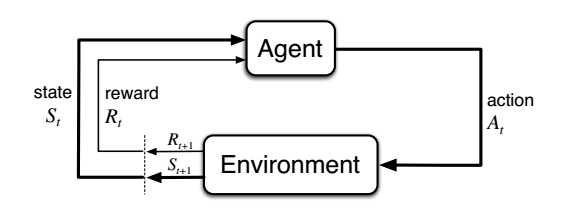
\includegraphics[width=350px,height=200px]{rl_diagram.png}
        \caption{RL}
        \label{fig:my_label}
    \end{figure}


"Reinforcement learning is learning what to do and how to map situations to actions so as to maximize a numerical reward signal" Sutton (pg 1)

A full discussion of reinforcement learning is not required to understand AlphaGo Zero but it is necessary to define terminology that is used in the paper. 

    \begin{enumerate}
        \item Environment
        \item State
        \item Policy
        \item Reward Signal 
        \item Value
        \item Model
    \end{enumerate}
    
    \subsection{Environment}
    
    Loosely defined as the thing that the agent interacts with. Everything that is exterior to the agent. The environment typically encompasses the system that is trying to be solved. It also provides observations and rewards as the agent takes actions. For example when trying to solve the game of Go the agent (the players) takes actions (moves pieces) and the environment is the board, the pieces, and the mechanism for telling the agent the current reward (win / loss) or other special states that are specific to the game. So it is the game itself plus a few other mechanisms to make the learning process possible. The environment is not synonymous with state as observed by the agent. We will look at that next. 
    
    \subsection{State}
    
    State is the representation of all information that is available to the agent at any given time. As said above this is not necessarily the same as the observation provided by the environment. For instance in AlphaGo Zero we will see that the state is actually a function of the current board as well as previous board positions. It is up to the designer of the reinforcement learning algorithm as to what is the best state to present to an agent. In many environments the choice might be more obvious than others. 
    The fact that state is something that needs to be decided upon by the designer of the algorithm hints at a potential need for more generalization within algorithms. MuZero and similar algorithms take a step in this direction by having the agent learn that representation. MuZero as will be discussed towards the end of this paper searches in a latent space. So the state as provided by the environment is projected onto a latent space and then the algorithm searches within this space. This is an interesting approach. For further discussion on this see \cite{predictron,muzero}
    
    \subsection{Policy}
    
    A policy roughly speaking is just a definition of an agents behavior given a perceived state of the environment. That is it is a mapping $ \pi: s \rightarrow a $ where s is a state of the environment and a is an action  $ a \epsilon A $. A is the possible set of actions the agent can take. It can be either discrete or continuous. In AlphaGo Zero actions are integers representing the place on the board.
    
    \textbf{Note} The Environemnt typically has to tell the agent when a move is illegal. So that in some way that action can be discarded from the possible set of actions to take. Again this opens up opportunity for generalization as the agent is dependent on a correct model of the environment in most algorithms. MuZero is an example of an algorithm that gets around this constraint by learning its own model and learns an internal representation of when actions are impossible. 
    
    \subsection{Reward Signal}
    
    A reward signal is what defines the goal of a RL algorithm. As an agent observes an environment it receives feedback in the form of rewards. Generally an agent is simply trying to maximize the sum of its reward over the long run. Rewards help the agent to learn a policy. An agent will adjust the actions that it takes based off of the feedback it receives. Roughly speaking the agent will adjust to take actions more frequently that it perceives to return more reward. In environments like AlphGo Zero there is what is called the "sparse rewards" problem. This means that the agent might be interacting with the environment for long extended periods of time before receiving any feedback. 
    
    \textbf{Note} Another opportunity for generalization is here. It seems that biological systems although of course receiving true feed back from the environment also have their own interpretation of that feedback. Algorithms that have their own model or internal representation for rewards may be able to solve sub tasks more effectively. For example in Go making it to a favorable board position might elicit some reward. Of course a counter argument to this would be that a good value function should handle this by finding those board situations are valuable. A value function needs actual feedback from the environment to be learned and so perhaps a sort of separation of tasks could help inform the overall system. 
    
    \subsection{Value}
    
    The value of a state in reinforcement learning is the amount of reward an agent should expect to receive in the long run from a given state. An agent is not given this number and is something that needs to be learned. This is generally expressed like this $ V(s) \rightarrow \mathbb{R} $. 
    
    From Sutton
    $ v_{\pi}(s) = E_{\pi}[G_{t}| S_{t} = s]$
    
    
    \subsection{Model}
    
    A model from the perspective of RL typically refers to a predictive model of the environment. It is a way for the agent to predict the behavior of the environment. This allows the agent to make inferences about what will happen when certain actions are taken. This in turn allows the agent to plan based on the model. Algorithms that use models are called \textit{model-based}. Algorithms that dont explicitly model the environment are called \textit{model-free}. The line between the two can easily become blurred as a lot of algorithms will mix between the two approaches. In the context of this paper AlphaZero and can be viewed as a Model free algorithm and MuZero as a model based extension to AlphaZero. MuZero attempts to learn the dynamics of the environment from scratch whereas for AlphaZero the dynamics are known upfront.  
    
\section{Self-Play}

Self-play is a concept that has been around in AI for a long time depending on how liberal your willing to be with the term AI. In 1951 Brown came out with a paper describing fictitious play a self-play algorithm In 1959 Checkers was solved using self-play with expert knowledge. There have been many other successes including AlphaZero. Self-play in short is any algorithm for which there are 2 or more players and the agent makes actions for every player. So the agent just plays against itself and improves play based off of what it observes during this self-play. This is easiest to see in zero sum two player games since they are symmetric. In this setting a self-play algorithm will play as both player 1 and player 2.The agent will play against itself switching perspectives between player 1 and player 2. AlphaZero does just this. We do this as humans occasionally when playing a game or perhpas other activities. For instance when thinking about how to develop better chess strategies you might see how well a strategy does by attempting to play against that strategy yourself and observing the outcome. 

\section{Markov Decision Processes}

The following section draws pretty heavily from Sutton. Lets put some of the previous concepts together into a framework that we can actually use to make decisions. Markov decision processes (MDP) are an idealized environment for making sequential decisions. MDPs have been studied quite thoroughly and although their formulation is simple it is also quite robust and a surprisingly large number of problems can be formulated as MDPs. Figure 2.1 that we looked at before is an example of a MDP. What kind of data would we get if we allowed the process in that figure to go on for many time steps? First the agent begins in the start state $S_{0}$ and takes action $A_{0}$ and receives a reward $R_{1}$ and the next state $S_{1}$. Then the agent would take another action $A_{1}$ and so on. This would result in a series of data points $S_{0},A_{0},R_{1},S_{1},A_{1},R_{2},S_{2},A_{2}....R_{T},S_{T}$. Here there is some terminating condition at time $T$ but the series could also just go on continuously. $R_{t},S_{t}$ are both random variables whose probability of occurrence only depends on the previous action and reward. This is what makes the process markovian and is called the Markov property. The only thing that matters in determining the probability of the next state and reward is the current state and action. The dynamics of this process can be described by a function $p: S x R x A x S \rightarrow [0,1] $. The function can be defined in terms of conditional probability. 

$$ p(s^{'},r | s, a) = Pr\{S_{t + 1} = s^{'}, R_{t + 1} = r | S_{t} = s, A_{t} = a\}$$

So the probability given by $p$ describes the entire environment dynamics. The Markov property as described in Sutton {Introduction to reinforcement learning} "is best viewed as a restriction not on the decision process, but on the state. The state must include information about all aspects of the past agent–environment interaction that make a difference for the future".

How state, action and time is defined is quite flexible in this formation. Time does not have to refer to an actual interval of time but can just be some set of steps that happen one after the other. Actions likewise can really be any decision that we want to learn how to make. 

Now that we have defined the system what is the actual goal? We want to get as much reward as possible. That means no just the reward that we receive right now but all the reward we accumulate. This statement results in the \textit{reward hypothesis} {Introduction to reinforcement learning}

\say{..what we mean by goals and purposes can be well thought of as the maximization of the expected value of the cumulative sum of a received scalar signal (called reward)}.

Since learning from rewards has become so popular it might not seem like that strange of a concept and indeed it might be fairly intuitive. However this is one of the things that distinguishes reinforcement learning from other forms of machine learning. In a typical supervised learning setting for instance you attempt to minimize a loss function on a set of observed data w.r.t to some given labels. Like attempting to predict credit card fraud from a set of features. You are first given a bunch of examples with labels as to whether fraud occurred in that particular instance. You then want to train a model to be able to generalize from these observed features and labels to unlabeled or data that has not been seen yet. Reinforcement learning is different in that we dont generally start out with a set of features and labels. The agent produces data or observation as we act in the environment. Then through these observations we change the agents behavior as to achieve a desired goal. There is a bit of an art in setting up the rewards correctly. The designer of the algorithm has to choose the rewards for an environment and it is not always trivial. For GO and other two player zero sum games it is natural to assign a reward of +1 for winning, -1 for losing and 0 for a draw. You might however want to assign a small amount of reward to a draw so that the agent is receiving some amount of feedback. You might want to set up intermediate goals as to "show" the agent the right choices to make or steer them away from obviously bad choices. An example of a miss application of reward assignment would be in chess to give reward to an agent for pieces captured. This can lead the agent to commit detrimental errors to the main goal of winning just to achieve the sub goal so care must be taken that the subgoals align with the main goal. 

In this paper we will be focused on situations in which there is a clear start and end state. There are of course other domains in which this is not the case. Self-driving cars, trading in markets, and playing atari games are a few examples. Since we are trying to maximize an accumulated reward we can define our main goal as the following. 

\begin{equation}\label{Cumulative sum}
 G_{t} = \sum_{k=t + 1}^{k=T} R_{k}
\end{equation}

There is something still not quite right here. In this formulation we would value rewards at all time steps equally. This is usually not the case in most tasks however. The idea that 100\$ today is better than 100\$ 10 years from now applies here. Typically the reward we get now is more valuable then the same amount in the future. So we can modify our goal a bit by discounting rewards that we receive farther into the future. We do this by using a discount factor $\gamma < 1$. 

\begin{equation}\label{Discounted Cumulative Sum}
G_{t} = \sum_{k=t + 1}^{k=T} \gamma^{k - t + 1} R_{k}
\end{equation}

Ok, great we have a goal now how do we use that goal to start defining how the agent is going to behave? Well we want the agent to take actions that are going to lead to higher $G$. Taking actions in our MDP formulation leads us to end up in different future states. So we want to end up in better states. What does it mean to be a better state? A better state is one that leads to more $G$. So we want to be in states in which we expect to collect more reward in the future. Lets try and put this into something concrete. The expected value of a state seems to fit well into what we are going after so we can use that as a starting point. 

\begin{equation}\label{Expected State Value}
\mathbf{v}_{\pi}(s) \dot{=} \mathbb{E}_{\pi}[G_{t} | S_{t} = s]
\end{equation}

The $\pi$ here refers to the policy of the agent. So this is looking at the expected value assuming the agent is following a given policy. We discussed policies previously and we will discuss them more in the future. It is important for knowing the expected value while following an MDP because a policy will define how we transition from one state to the next. We can also define a value function for a state action pair in a similar manner. 

\begin{equation}\label{Expected State Action Value}
\mathbf{q}_{\pi}(s,a) \dot{=} \mathbb{E}_{\pi}[G_{t} | S_{t} = s, A_{t} = a] 
\end{equation}

Its quite easy to see that if one actually had access to one of these functions how you might have the agent behave. In the case of $\mathbf{q}_{\pi}$ simply pick the action with the largest value. We of course don't have access to these and have to learn them from experience. How might we do this? One way is to somehow track the average return that you get from a particular state or state action pair. This approach is called Monte Carlo methods. This is quite relevant for understanding AlphaZero as a form of tree search called Monte Carlo tree search is central to the algorithm. 
    
One central idea in reinforcement learning is the ability to view a value function recursively. Lets look at how we can do that. First we can write our cumulative variable $G_{t}$ in terms of the next immediate reward and a discounted cumulative return starting from the next timestep.  

    $$ \mathbb{E}_{\pi}[G_{t} | S_{t} = s] = \mathbb{E}_{\pi}[R_{t + 1} + \gamma G_{t + 1} | S_{t} = s] $$
    
Then we can expand this by thinking about what en expectation means here in terms of our random variable $R_{t + 1}$. In words it is the value of all future rewards we would see by transitioning to new states. We have said previously that the probability of transitioning to a new state $s^{'}$ and receiving reward $r$ from the current state given a certain action is given by the function $p(s^{'},r|,s,a)$ the system dynamics of our MDP. We know the definition of expected value is the sum over possible outcomes of a random weighted by the probability of that outcome happening. So we can write the expected value of $R_{t}$ given a specific state and action. 

$$ \mathbb{E}[R_{t}] = \underset{s^{'},r}{\sum}p(s^{'},r|,s,a)[ r ]$$

We want however to look at the expectation following a specific policy. A policy $\pi(a|s)$ gives us a distribution over possible next actions given the current state. So we can further expand on our previous equation. 

$$ \mathbb{E_{\pi}}[R_{t}] = \underset{a}{\sum}\pi(a|s)\underset{s^{'},r}{\sum}p(s^{'},r|,s,a)[ r ]$$

We can now go back to our expectation of the cumulative reward. 

$$\mathbb{E}_{\pi}[R_{t + 1} + \gamma G_{t + 1} | S_{t} = s] = \underset{a}{\sum}\pi(a|s)\underset{s^{'},r}{\sum}p(s^{'},r|,s,a)[ r + \gamma \mathbb{E}_{\pi}[G_{t + 1} | S_{t + 1} = s^{'}]] $$

Notice how the expectation is now conditioned on the next state. This allows us to rewrite this in a recursive form.

\begin{equation}\label{Bellman State Value Equation}
\mathbf{v_{\pi}(s)} = \underset{a}{\sum}\pi(a|s)\underset{s^{'},r}{\sum}p(s^{'},r|,s,a)[ r + \gamma \mathbf{v_{\pi}(s^{'})}]
\end{equation}

This last form is know as the bellman equation. The bellman equation represents values of a state in terms of values of future states. The figure below taken from Sutton represents this as a decesion tree. The open circles are states and the black circles are actions. This shows if you are in state $s$ you have 3 actions that are part of policy $\pi$. Once you take one of those actions the environment then transitions to one of two next states $s^{'}$ and emits a reward $r$ with probability $p$. You could then extend the diagram in the same way from each of the next states. If this were a two player game the other player would be part of the environment and the probability of transition to state $s^{'}$ would depend on the other players policy $pi$. Sutton refers to these as backup diagrams because they show how information could be propagated back up the tree. 

\begin{figure}[h!]
        \centering
        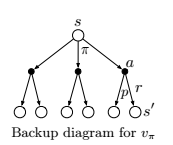
\includegraphics[width=350px,height=200px]{images/bellman_update.png}
        \caption{RL}
        \label{fig:my_label}
\end{figure}

We have now discussed how to evaluate given states within our framework. We have not discussed yet how to actually use this information to make good decisions. There is a theorem in RL that says that a policy $\pi$ is better than or equal to another policy $\pi^{'}$ if its expected value is greater than or equal to the expected value of $\pi^{'}$ for all states. In other words $ \pi \geq \pi^{'} $ iff $ \mathbf{v_{\pi}}(s) >= \mathbf{v_{\pi^{'}}}(s)$ for all $ s \in  S$. It has also been shown and we will restate here without proof that an optimal policy always exists for an MDP. There can be more than one but at least one exists. The notation used for the optimal policy is usually $\pi_{*}$ and we will take that notation here as well. This leads also to the fact that there is an optimal state value function. 

\begin{equation}\label{Optimal State Value Equation}
\mathbf{v_{*}}(s) \dot{=} \underset{\pi}{max} \: \mathbf{v_{\pi}}(s) , \: \forall s \in S 
\end{equation}

The bellman equation representation must hold as well. In our previous representation of the bellman equation we had to some over all actions from our policy $\pi(a |s)$. When looking at an optimal policy in the case of an MDP we will only be interested in taking the best action. So we can rewrite the bellman equation of the value function with that in mind. 

\begin{equation}\label{Optimal Bellman State Value Equation}
\mathbf{v_{*}}(s)= \underset{a}{max}\underset{s^{'},r}{\sum}p(s^{'},r|,s,a)[ r + \gamma \mathbf{v_{*}(s^{'})}]
\end{equation}


A similar analysis can be done for $q(s,a)$. We will not go through that here but you can look to Sutton or other sources for more discussion. 

\begin{equation}\label{Optimal Bellman State Action Value Equation}
\mathbf{q_{*}}(s,a)= \underset{s^{'},r}{\sum}p(s^{'},r|,s,a)[ r + \underset{a}{max} \: \mathbf{q_{*}}(s^{'},a^{'})]
\end{equation}

I think that the $\mathbf{q_{*}}$ optimal value function can be more intuitive. It simply says that the value of the optimal action from the current state is a weighted sum over possible next states assuming we take the optimal action from those states as well. If you have $\mathbf{q_{*}}$ or $\mathbf{v_{*}}$ than coming up with the correct policy is easy. For $\mathbf{v_{*}}$ you just have to do one step look ahead to see which actions will give you the max. You dont have to continue to look further because you already have access to the optimal values of the next state. With $\mathbf{q_{*}}$ you simply look up the best action from the current state. No further search is necessary. Obtaining these optimal functions of course generally takes a lot of work and in any large setting is intractable to compute directly. To actually compute an optimal bellman equation you need to have perfect knowledge of the environment, sufficient resources and the markov property. These assumptions typically dont hold for most interesting problems. For any problem that breaks one of these assumptions some sort of approximation will be needed. One approach that fits in closely with the bellman optimality equation is dynammic programming which we will discuss shortly. One big takeaway from reading Sutton and others work is that most reinforcement learning techniques come down to different ways of approximating the bellman optimality equation. To me this is quite powerful and means that even though we might come across some powerful approximation techniques such as those that we see in AlphaZero they can all be viewed from the perspective of approximating the bellman equation in some way. 

\section{Dynamic Programming}

Dynamic programming (DP) is one of the more foundational topics within machine learning. We will not dwell on this topic too long but there are a few important lessons in which DP can help inform our understanding of RL and AlphaZero. We have just concluded discussing optimal value functions and now we need to find a way to actually compute them. That is where DP comes in. DP is essentially a collection of algorithms used to compute optimal value functions. Recall that (\ref{Bellman State Value Equation}) gave us a way to evaluate the value of state given a certain policy. This equation actually gives us a system of linear equations and can be solved directly if the model of the environment is totally known. We have $|S|$ equations and $|S|$ unknowns. This of course is not computationally very feasible so we need to find a way to compute (\ref{Bellman State Value Equation}) iteratively. We can actually just turn it into an update rule like the following. 

\begin{equation}\label{Bellman State Value Update Equation}
\mathbf{v_{k + 1}(s)} = \underset{a}{\sum}\pi(a|s)\underset{s^{'},r}{\sum}p(s^{'},r|,s,a)[ r + \gamma \mathbf{v_{k}(s^{'})}]
\end{equation}

We can first initialize $v_{0}(s)$ for each state randomly. We can use domain knowledge to set reasonable initial values as well or just set everything to 0 to start. This iterative process will converge to $v_{\pi}$ as $ k \rightarrow \infty$. This is called \textit{iterative policy evaluation} and it gives us a way to evaluate the current policy $\pi$ in an iterative fashion. We of course dont have to wait for $ k \rightarrow \infty$. In practice we can implement some stopping condition for which we are satisfied that $v_{k}$ is close enough to $v_{\pi}$. 

We dont want to just know the value of a given policy however we want to find what the best policy is. So we need to find a way to update our policy as well. I will state here what is known as the \textit{policy improvement theorem}. 

\newtheorem{remark}{Policy Improvement Theorem}

\begin{remark}\label{Policy Improvement Theorem}
Let $\pi$ and $\pi^{'}$ be any two separate deterministic policies for all $s \in S$ s.t. $q_{\pi}(s,\pi^{'}(a)) \geq v_{\pi}(s)$. Then the policy $\pi^{'}$ is greater than or equal to $\pi$. This implies that $ \forall s \in S$ each state value function has the relationship that $v_{\pi^{'}}(s) \geq v_{\pi}(s)$
\end{remark}

The idea here is that if you can take a policy $\pi$ and change one of its actions at a particular state to guarantee that it is at least as good or better than $\pi$ at that state then you can just change the policy at that particular state to the new action and you now have a better policy $\pi^{'}$. How can we do this at every state to give us a general methodology. We can do whats called acting greedily. Acting greedily means that from a given state you take the action that maximizes return from a one step look ahead perspective according to $v_{\pi}$. We can adjust (\ref{Bellman State Value Equation}) once again to represent this. 

\begin{equation}\label{Greedy Policy}
\mathbf{\pi^{'}} = \underset{a}{argmax}\underset{a}{\sum}\pi(a|s)\underset{s^{'},r}{\sum}p(s^{'},r|,s,a)[ r + \gamma \mathbf{v_{\pi}(s^{'})}] = \underset{a}{argmax} \: \mathbf{q_{\pi}(s,a)}
\end{equation}

This just says what we have already said in words. We use the current policy $\pi$ and take the action that is going to maximize our policy evaluation from a given state using $\pi$. This gives us a new policy $\pi^{'}$ that we know from the policy improvement theorem will guarantee us an improved policy. The only way its not an improvement once again is if we already had an optimal policy. Now that we have a new policy $\pi^{'}$ how can we continue to improve it. We need to evaluate $\mathbf{v_{'}}$ using policy evaluation. Then we can use (\ref{Greedy Policy}) again to get a new policy $\pi^{''}$

$$ \mathbf{\pi^{''}} = \underset{a}{argmax}\underset{a}{\sum}\pi^{'}(a|s)\underset{s^{'},r}{\sum}p(s^{'},r|,s,a)[ r + \gamma \mathbf{v_{\pi^{'}}(s^{'})}]
$$

We can then repeat this process until convergence. This algorithm is called \textit{}{policy iteration} and is given in full below. 

 \begin{figure}[h!]
        \centering
        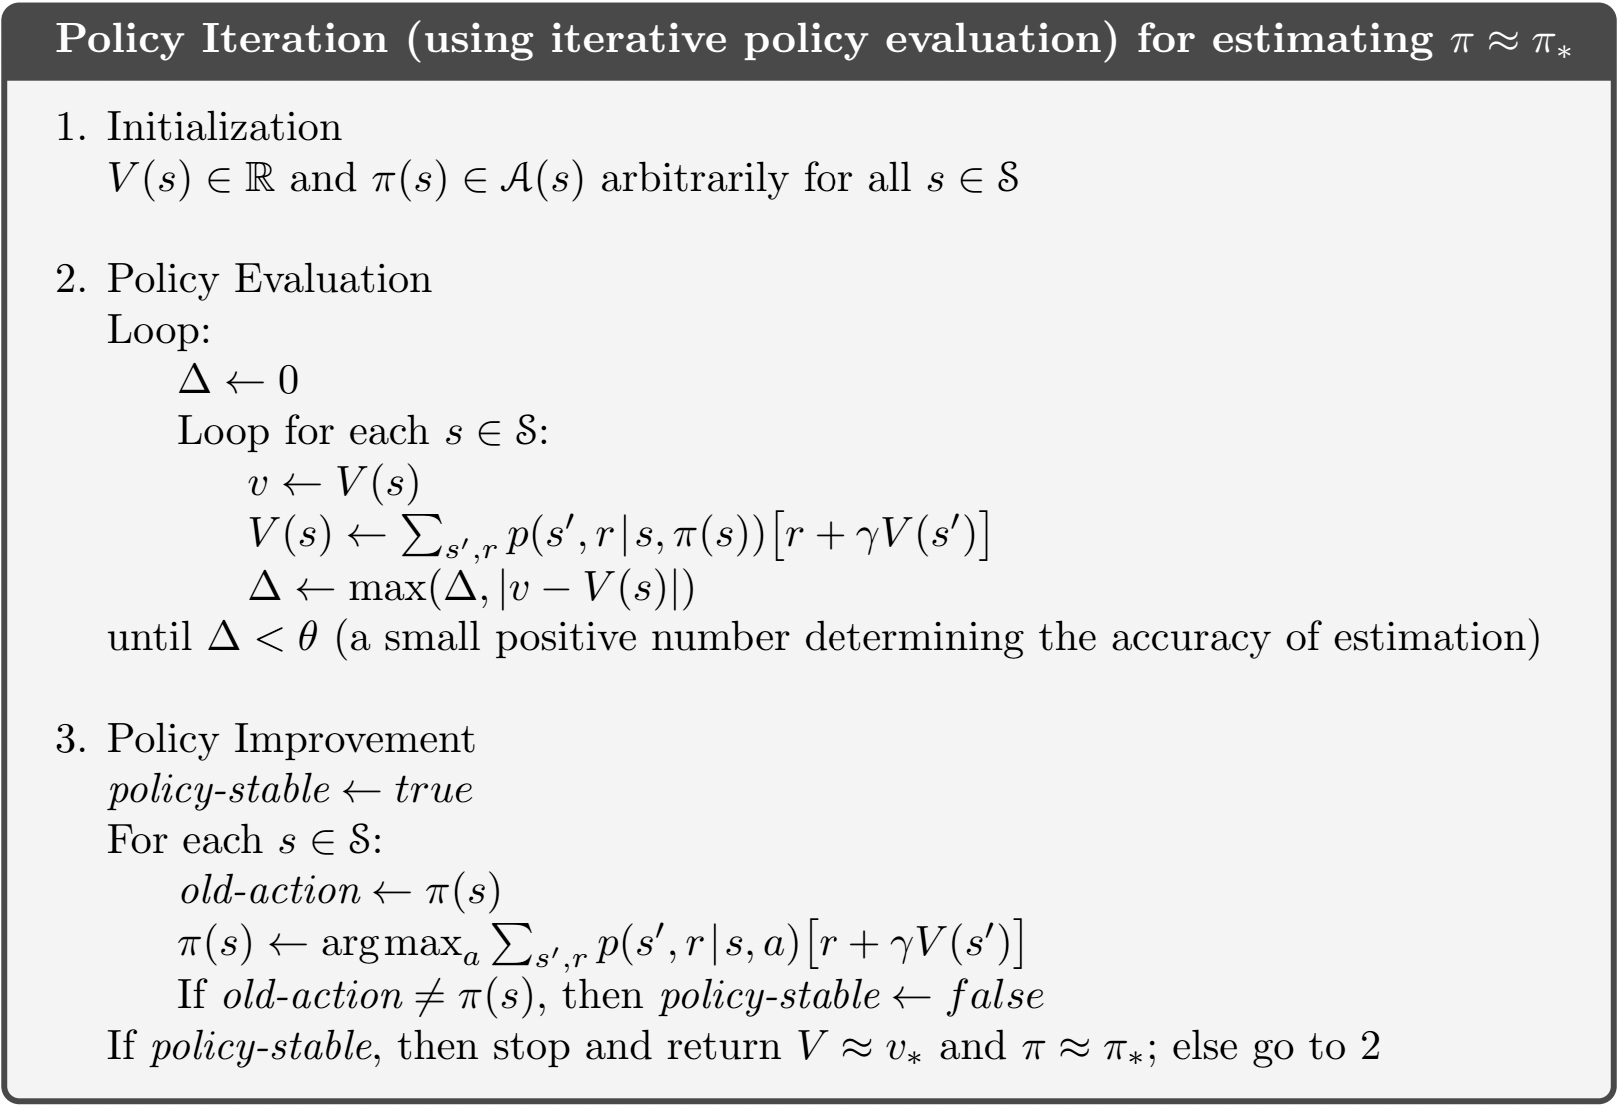
\includegraphics[width=350px,height=200px]{images/policy_iteration.png}
        \caption{From Sutton Chpt 4.3}
        \label{fig:my_label}
    \end{figure}

This idea of iterating back and forth between evaluation of a policy and improving a policy is a fairly general concept. In fact there is something called \textit{General policy iteration} (GPI) which captures these two concepts. Many reinforcement learning algorithms can be described in terms of GPI. The process is quite interesting because as soon as you perform policy improvement your value function is no longer accurate because it is still in reference to the old policy. So then you update the value function with the new policy to make it accurate again. The policy however is no longer optimal w.r.t the current value function so you adjust the policy by once again acting greedily. This goes back and forth until convergence is reached. There is a constant pushing and pulling between policy evaluation and policy improvement. 



\section{Monte Carlo Methods}

Monte Carlo in regards to reinforcement learning is a bit more specific than its typical meaning. In this discussion by "Monte Carlo" we mean any method that uses an average return for estimation. We will focus on estimating the value $\mathbf{v}_{\pi}(s)$ of a particular state. We said that our goal with $\mathbf{v}_{\pi}$ was to compute the expected value of the cumulative returns from a particular state. To apply monte carlo methods to this problem we can just track the average return we observe visiting that particular state. We can do this directly from experience assuming the agent is following the policy $\pi$ and in the limit we should have a true estimate of $v_{\pi}$. This is called Monte carlo prediction and the most common form is called first-visit. This means that we


\section{TD learning}

In this section we w